% results goes here. 
\subsection{Experimental Setup:}

The large scalability experiments reported in this paper were
performed on \Titan~and \Stampede. \Titan~is a Cray XK7 supercomputer
at Oak Ridge National Laboratory (ORNL) with a total of 18,688
nodes, each consisting of a single 16-core AMD Opteron 6200 series
processor, with a total of 299,008 cores. Each node has 32GB of memory.
It has a Gemini interconnect and 600TB of memory across all nodes.
%
%\Stampede~ at the Texas Advanced Computing Center (TACC), is a linux cluster consisting of 6400 computes nodes, each with dual, eight-core processors for a total of 102,400 available cpu-cores. Each node has two eight-core 2.7GHz Intel Xeon E5 processors with 2GB/core of memory and a 3 level cache. Stampede has a 56Gb/s FDR Mellanox InfiniBand network connected in a fat tree configuration.
%(In addition, all of Titan's 18,688 compute nodes contain an NVIDIA Tesla K20 graphical processing unit, which we don't use currently). 
%\Stampede~ at the Texas Advanced Computing Center (TACC), is a linux cluster consisting of \textsc{6400} computes nodes, each with dual, eight-core processors for a total of \textsc{102,400} available cpu-cores. Each node has two eight-core 2.7GHz Intel\textsuperscript{\textregistered} Xeon\textsuperscript{\textregistered} E5 processors with 2GB/core of memory and a 3 level cache. Stampede has a \textsc{56Gb/s} FDR Mellanox InfiniBand network connected in a fat tree configuration.
%
\Stampede~  is the flagship supercomputer at the Texas Advanced
Computing Center (TACC), University of Texas at Austin. 
%It has $4,200$ Intel Xeon Phi 7250 (KNL) compute nodes, each with 96GB DDR4 RAM and 16GB of MCDRAM. 
It has $1,736$ Intel Xeon Platinum 8160 (SKX) compute nodes with $2\times 24$ cores and 192GB of RAM
per node. Stampede2 has a 100Gb/sec Intel Omni-Path
(OPA) interconnect in a fat tree topology. We used the SKX
nodes for the experiments reported in this work.


% \begin{figure}
% \hspace{-15 mm}
%     \centering
%     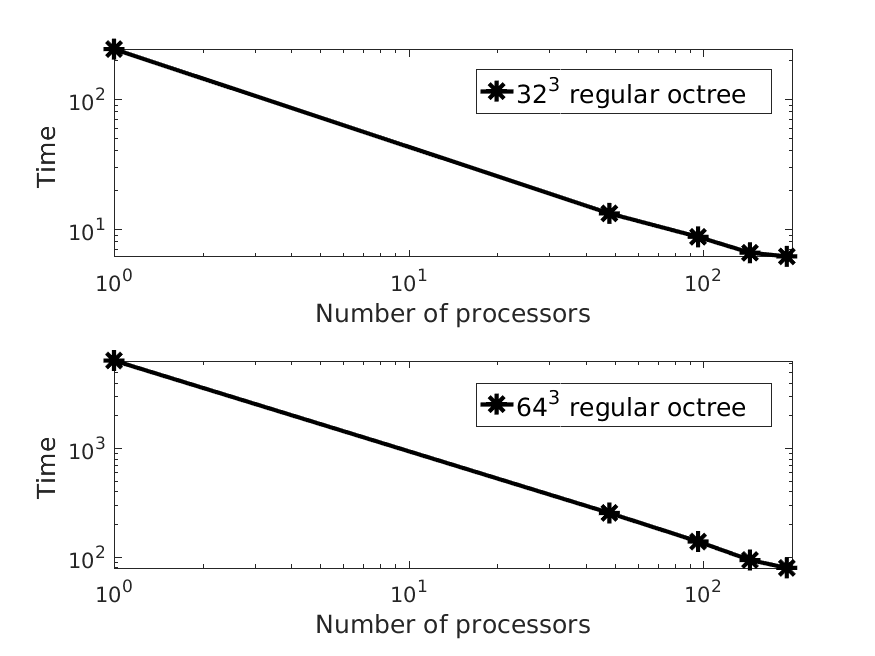
\includegraphics[scale = 0.5]{figs/Rtree.png}
%     \caption{Scaling of 3D + Backward Euler time stepping on TACC \Stampede~ SKX nodes for regular octree using matrix free method. The final time was set to be 1.0 s and the number of time step is equivalent to the number of the points in each direction.}
%     \label{fig:mfree_rtree}
% \end{figure}



\begin{figure}
    \centering
    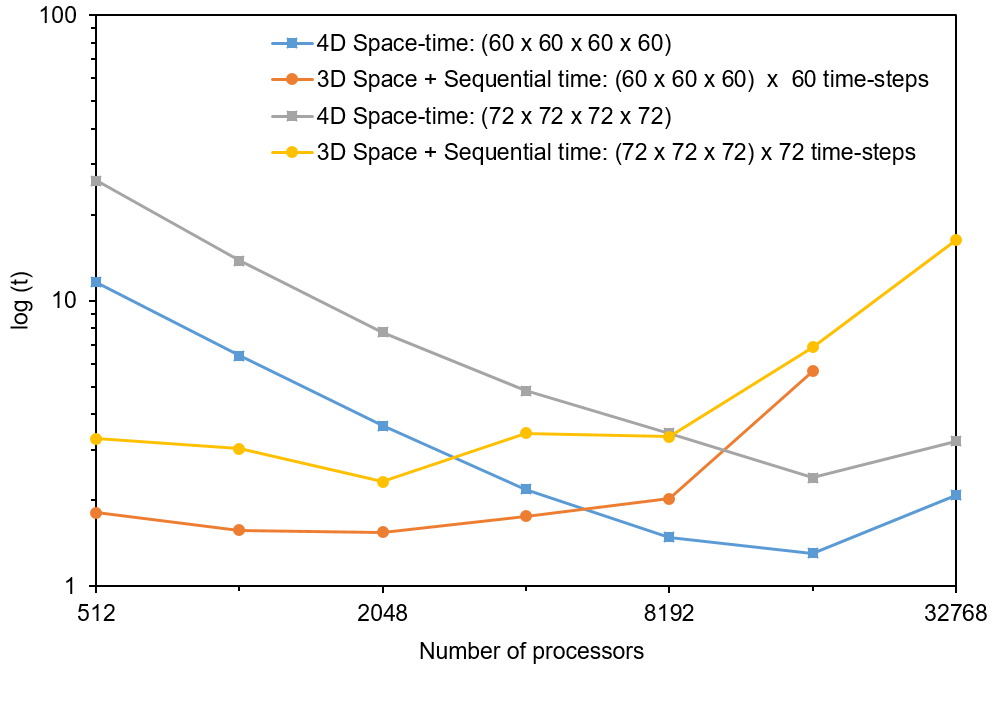
\includegraphics[scale = 0.5]{figs/solve-time-comparison-titan-TS-ST-linear-basis.png}
    \caption{Comparison of scaling of Crank Nicholson time stepping on Titan for linear diffusion problem with coupled space time formulation. The coupled space time formulation scales up to 16384 processors whereas the time stepping scales only up to 2048 processors. }
    \label{fig:comparison_Titan_4D}
\end{figure}

\begin{figure}
    \centering
    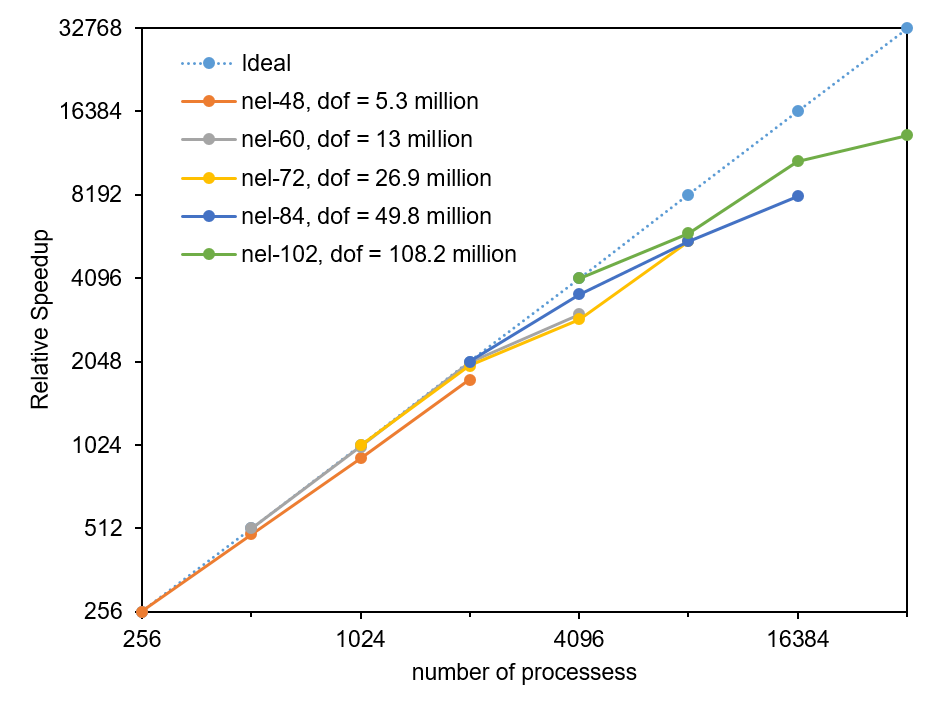
\includegraphics[scale = 0.5]{figs/scaling-titan-LIN-linear-nel-var-speedup.png}
    \caption{Relative speedup  of 4D space - time formulation on Titan. The number of degree of freedom was varied from 5.3 million to 108.2 million across 16384 processors.}
    \label{fig:matrix_Titan_4D}
\end{figure}


%  Then we solve the system using this forcing function (choosing the solution \textit{a priori} also allows us to calculate the analytical error in a suitable norm). %This solution is just an artificial solution chosen in the interest of numerical experimentation and should not be compared with a physically viable solution to the heat equation.
\subsection{Scalability}
We solve the linear diffusion equation \ref{eq:linearheat}, by artificially manufacturing the forcing function, with the given solution $u$ of the form:
\begin{align}\label{def:manufactured-solution}
    u(x, y, z,t) =  e^{t} \sin(\pi x)\sin(\pi y)\sin(\pi z)
\end{align}

Once we have the discrete bilinear form,  the problem is then translated into a linear algebra problem using $4D$ formulation as described in  \S\ref{sec:background} and \S\ref{sec:methodology}. The final linear algebra problem is solved using \petsc~ 3.7 via the \texttt{MATSHELL} interface to expose the mesh-free matrix-free interface. Figure \ref{fig:comparison_Titan_4D} shows the solve time comparison between a time stepping and a space-time problem on \Titan. The time stepping problem solves the PDE \ref{eq:linearheat} in a 3D spatial domain in a prescribed number of time steps through the well known Crank-Nicholson scheme. The space-time counterpart of this problem, is posed in a 4D space-time domain and is solved using the formulation presented in \S\ref{sec:background}. The space-time problem performs badly when the number of processors is low and in this region the time-stepping method is much more efficient. But as the number of processors increase we notice a linear decrease in the solve time for the space-time problem whereas the performance of the time-stepping method deteriorates slowly in the beginning and rapidly when the number of processors go above 5000. This shows concretely the potential of the space-time method with heavy parallelism. By adding the time dimension into the formulation, we are making the problem more complex from the point of view of computation, but this increased complexity in turn allows us to leverage the benefits of high parallelism. Indeed, when number of processors ~ 8000 and above then space-time formulation beats the sequential time stepping solution time.

Figure \ref{fig:matrix_Titan_4D} shows the relative speedup of the 4D space-time problem on  \Titan\ by varying the number of processors from 256 to 32768. The case with 102 elements in each direction (108.2 Million degree of freedom) scales up to 32768 processors. This is a strong scaling result and shows considerably good performance. It must be noted that this %is just the preliminary result with equal elements in each direction of space and time, and 
shows a very high potential to exploit the parallelism on the current scale of machines, which is not possible with the time stepping method. %Both of these cases were computed using the matrix version of the solver. 

We also present strong and weak scaling on \Stampede~ with a breakdown of times for different stages using linear and quadratic basis functions. In Figure \ref{fig:ws_stampede2}, we plot the weak scaling with breakdowns. we observe a dip in the communication costs for the $p=16$ case as this corresponds to a trivial partitioning in the $4D$ case, leading to very low communication costs. The influence on quadratic elements is less pronounced. Our current implementation is not very efficient with memory reuse during the bucketing leading to a significant cost for memory allocations. We are changing this by using a memorypool that should alleviate this problem. Similarly we present strong scaling results in Figure \ref{fig:ss_stampede2}. Again, we see excellent strong scalability for both linear and quadratic basis for a $64\times$ increase in parallelism. 

We are working to get larger runs through the queue on \Titan~ and \Stampede~ and expect even stronger results for larger problems. We expect to have these runs completed before the second round of reviews.